\section{各架构对应的芯片型号}

大家好，在本文章中我们将深入探讨不同GPU架构与其特定芯片之间的关联。需要指出的是在每个NVIDIAGPU架构内部都会发
布一系列芯片，每颗芯片可能具有独特的规格，但它们都共享相同的底层架构。以Ampere架构为例如本图所示，Ampere架构
包含多款芯片，如GA100、GA102等。这些芯片名称中的字母A代表Ampere架构。因此，这些芯片中的每一颗都可用于构
建面向不同市场细分的GPU。

\subsection{GA100芯片与高性能计算}

例如GA100芯片用于构建A100 GPU，这是超级计算机和高性能计算服务器中最知名的GPU之一。你可以在techpower up网站上验证这一信息。我们打开A100GPU的页面，这里列出的芯片名称就是GA100。如果你搜索该GPU的产品系

列，会发现它被归类于Tesla系列。而正如我们在前几期文章中多次讨论的，Tesla系列专用于高性能计算服务器和超级计算机
，这一分类清楚地说明了为何GA100芯片常被用于构建高性能计算HPCGPU。

\begin{figure}
    \centering
    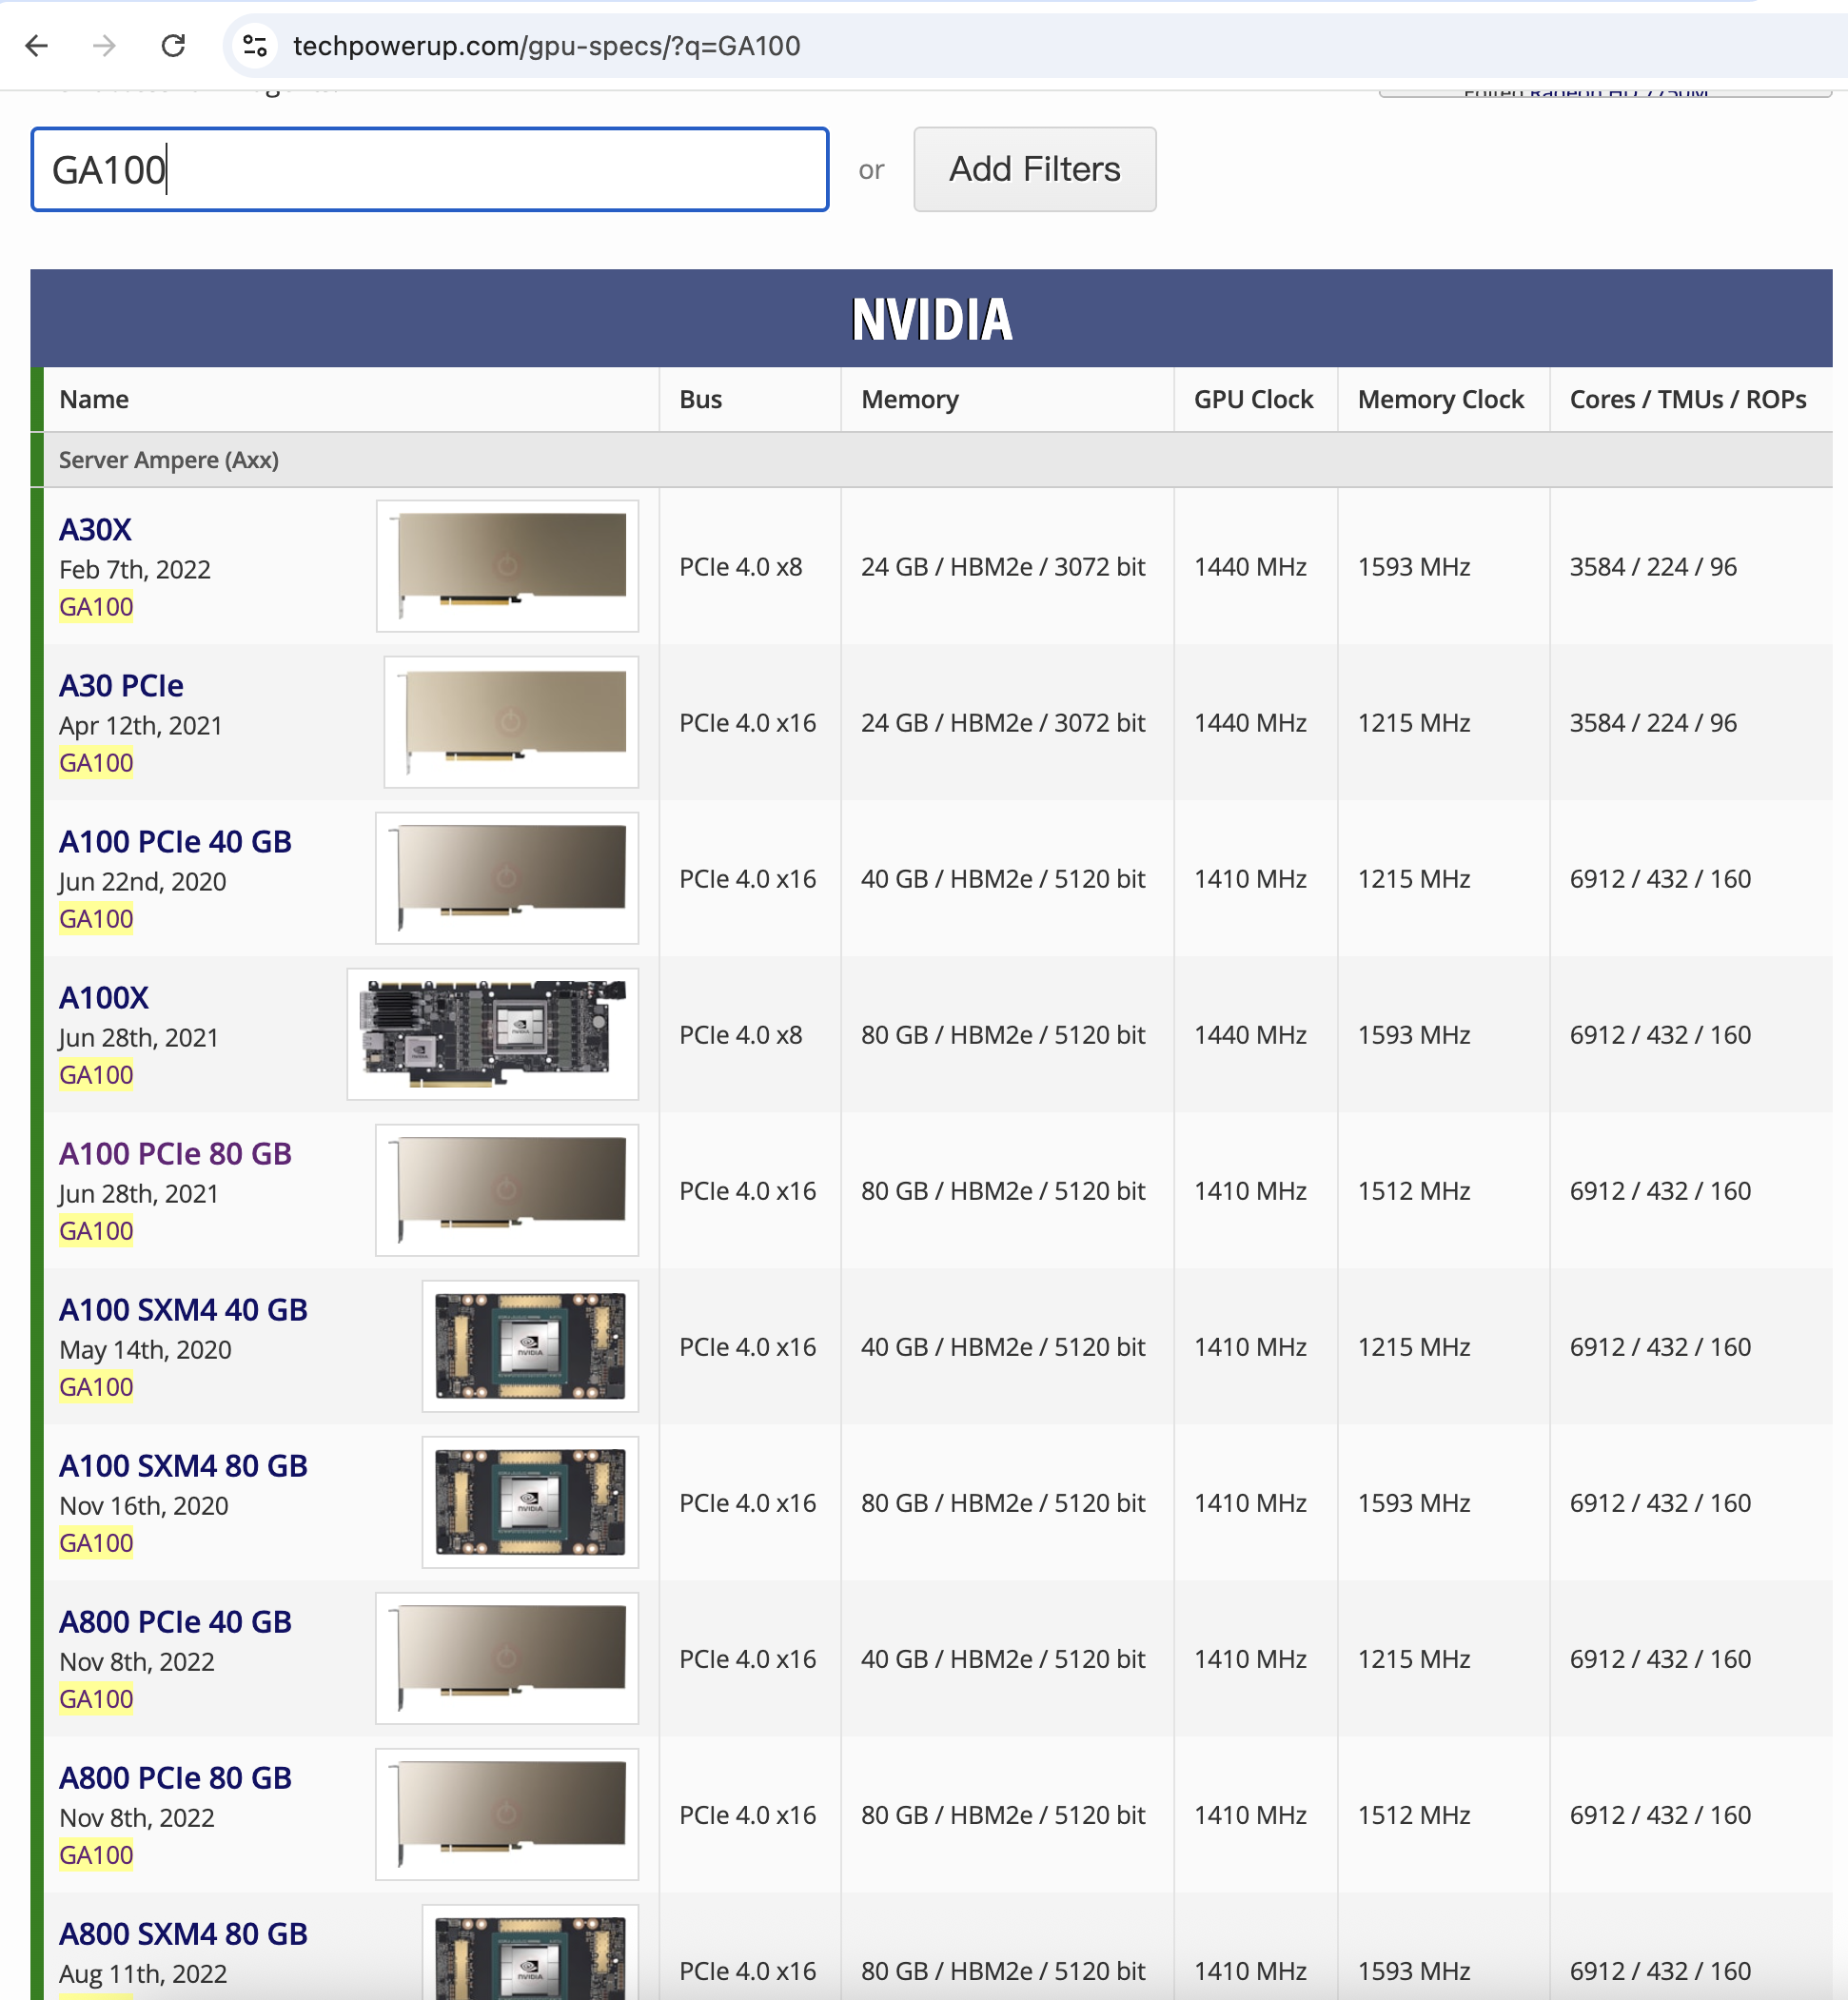
\includegraphics[width=0.75\linewidth]{resources/cuda-020.png}
    \caption{GA100}
    \label{fig:placeholder}
\end{figure}

\subsection{GA102芯片与消费级市场}

另一方面，我们的第二个例子，GA102芯片则更常用于面向普通用户或游戏玩家的GPU。例如该芯片出现在GeForceRTX
系列中专为普通PC或工作站设计。此外，从tech powerup网站这里的这一部分可以看出，这里的大多数GPU都带有散热
风扇。这是一个视觉标志，表明这些GPU是为日常使用设计的，而非用于高性能计算或超级计算机。

\begin{figure}
    \centering
    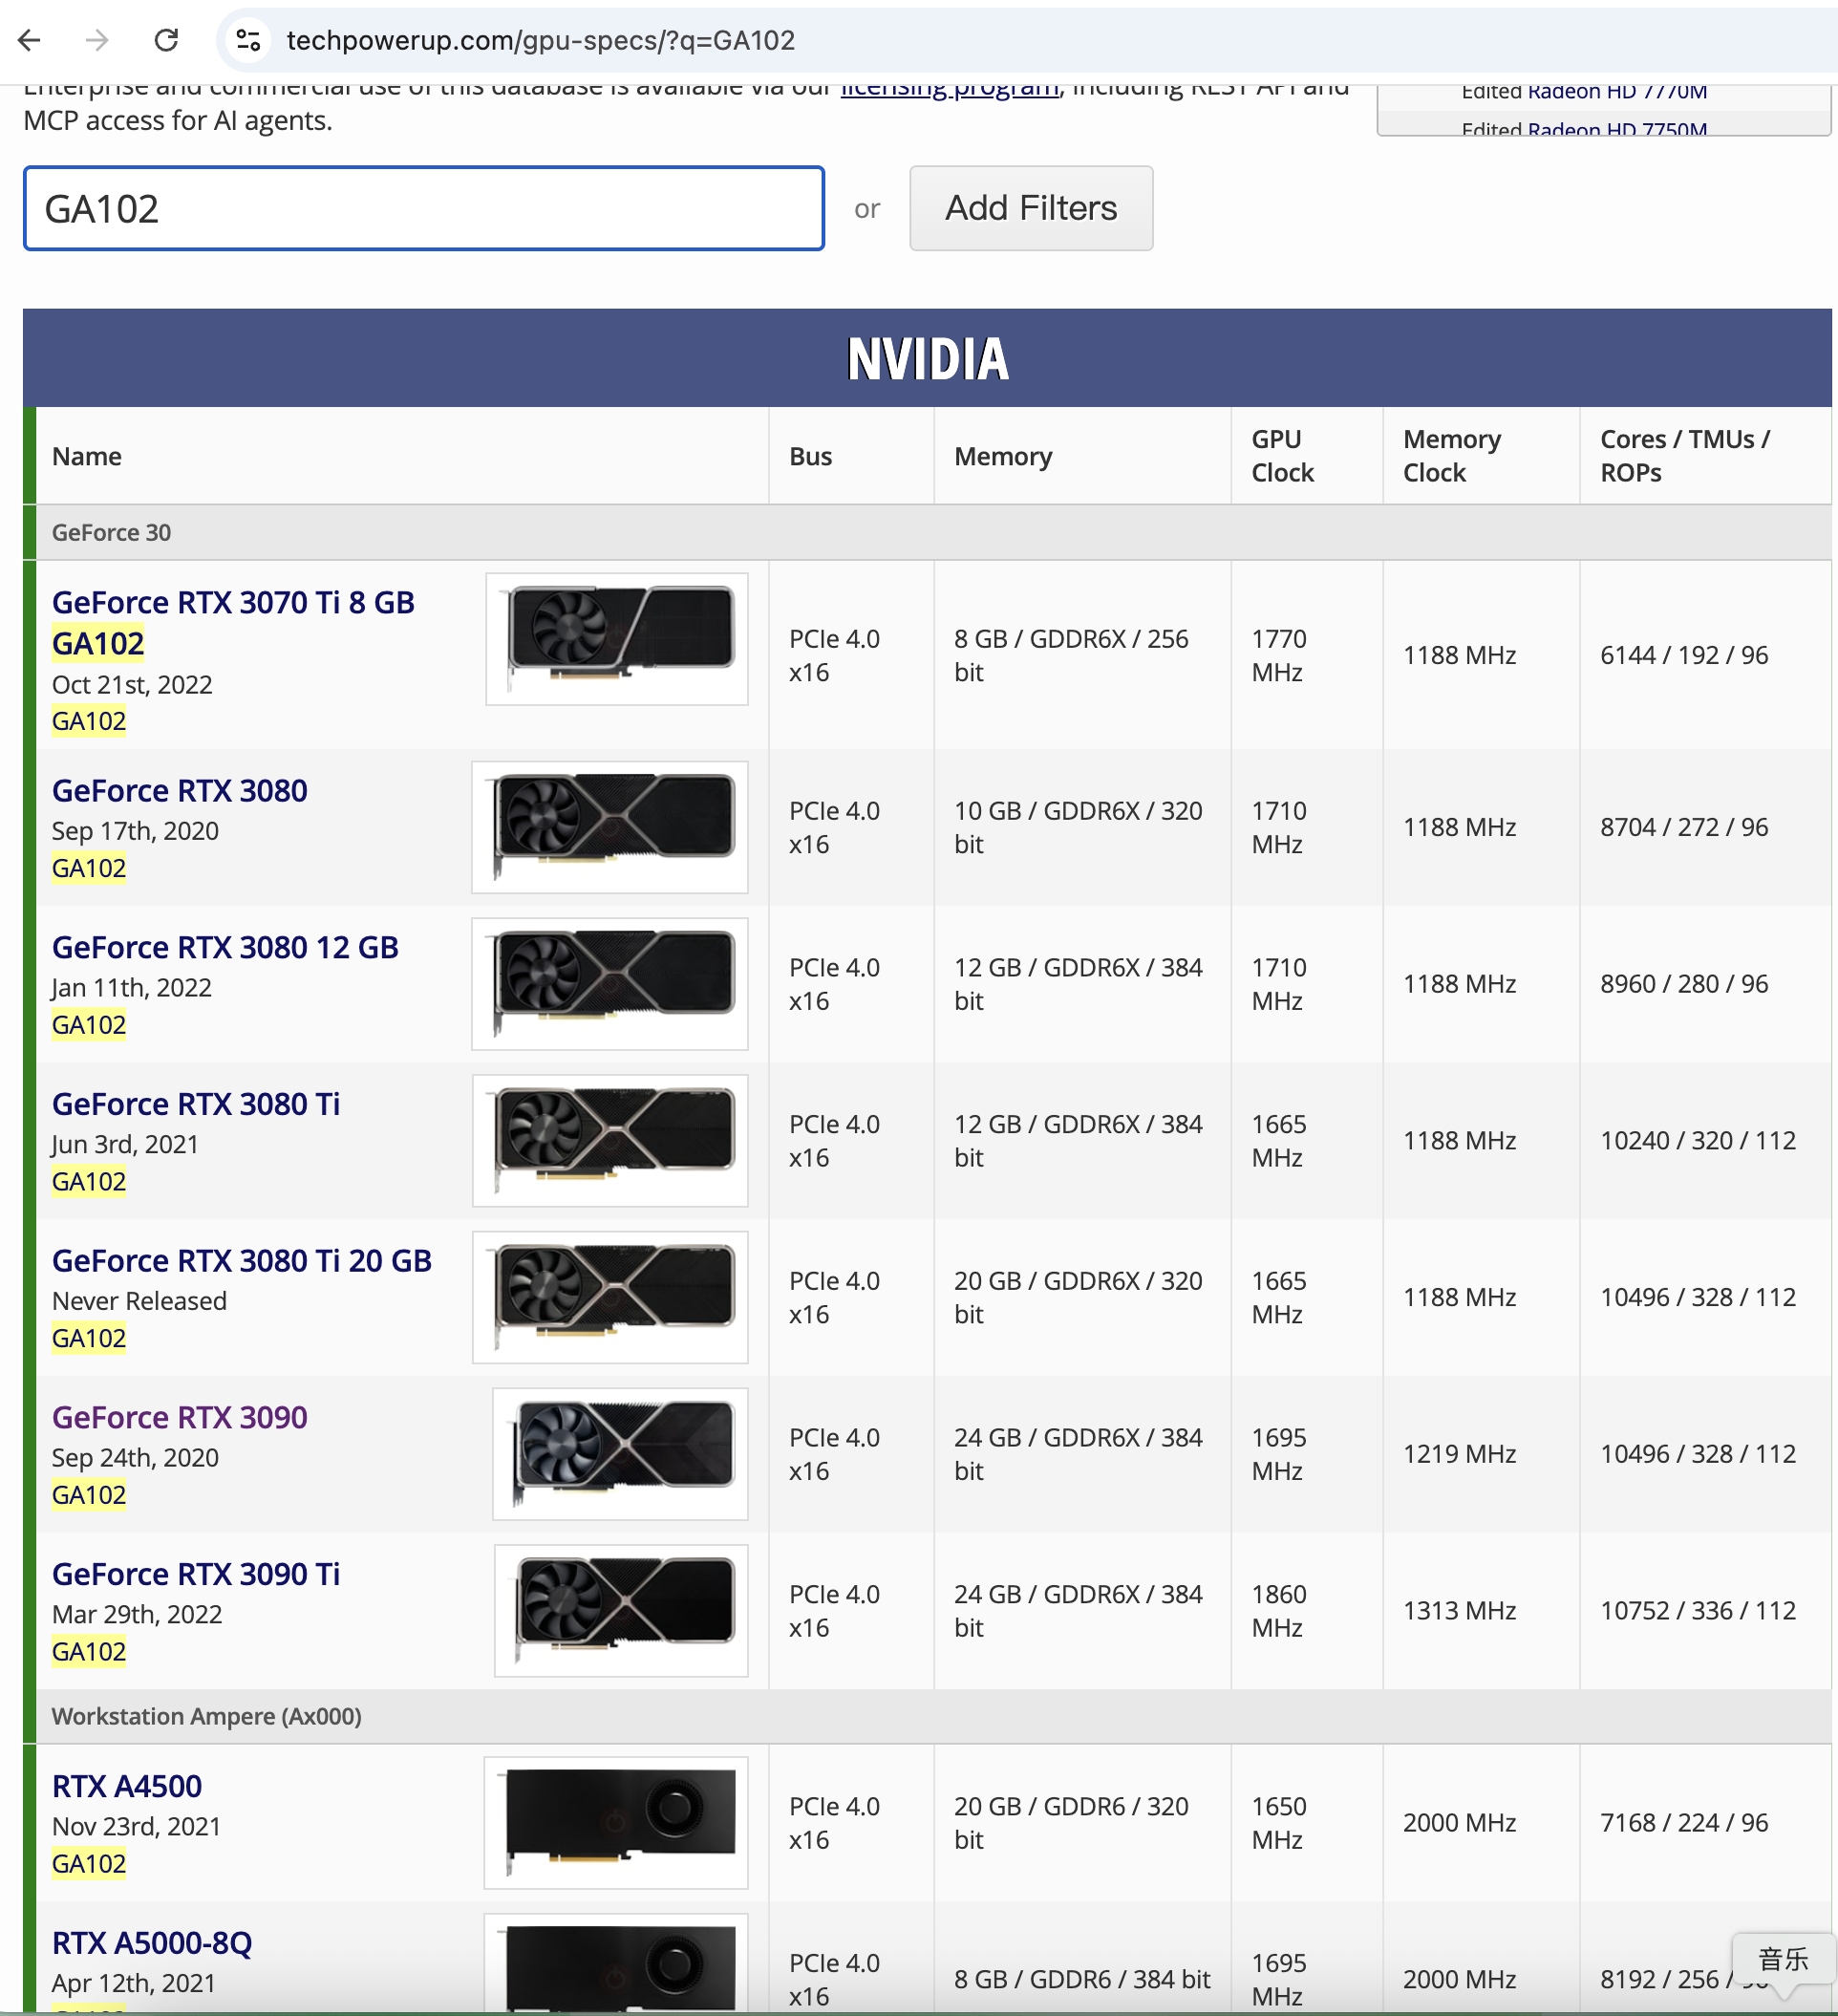
\includegraphics[width=0.75\linewidth]{resources/cuda-021.png}
    \caption{GA102}
    \label{fig:placeholder}
\end{figure}


同样的，如果我们再回到GA100芯片的网页，你会发现它通常用于不带散热风扇的GPU。这表明它被应用于超级计算机和高性能计
算服务器。这些场景通常采用其他更坚固的散热方法或系统，不过这并非总是如此。总结来说，现在已经很清楚某些芯片是专门为高性能
计算应用设计的，而另一些则是为日常消费级用途设计的。

\subsection{芯片的多用途适配}

NVIDIA有时会发布同一芯片的不同版本。例如，以Ampere架构中的一款芯片为例，我们以GA102为例，在其网页上我们
注意到它常用于游戏市场，因为大多数GPU都带有散热风扇，或者你可以打开其中一款GPU搜索其产品系列，结果应该是GeForce。例如，然而，如果我们查看该表格的前几行、前2或3款GPU，会发现这款芯片也被用于设计和制造高性能计算服务器用的GP

U。仔细查看此处这一部分，会发现这是GA102芯片的一个不同版本。它被称为面向高性能计算的版本。这款面向高性能计算的版本
编号为890，而面向游戏市场的版本编号则在100到350之间。

这展示了NVIDIA在将芯片适配多种用途方面的灵活性。我还想强调一点，值得注意的是，每颗芯片以及特定架构内的每个芯片版本
，都可能根据GPU型号甚至制造商的不同，以不同的速度或频率运行。这是因为NVIDIA会向市场上的多家公司提供GPU芯片和
授权，由他们生产GPU，这些公司生产的GPU可能在频率等细节上略有差异。

在本文章的最后，我想再次澄清，我在本课程中的目标是赋予你们独立处理这些主题的知识与技能。请记住，牢固的基础是掌握任何学科
的关键，这可以通过扎实掌握基础知识来实现。正如我们在本期文章以及之前文章中所探讨的内容。
